\chapter{Scientific Problem}
\label{section:scientificProblem}

\section{Problem definition}
\label{section:problemDefinition}
The purpose of the research in this thesis consists in approaching some alternative methods to replace classic file scanning techniques. Particularly, our target is to demonstrate that Machine Learning algorithms can be used as an efficient mechanism for malicios PDF files detection. Additionally, we want to present a framework that can remotely analyze suspicious PDF files by applying earlier mentioned performant algorithms. This framework has several advantages: 
\begin{itemize}
    \item Takes on the complicated task of applying classification model for uploaded files and giving the analysis result to the users.
    \item It is designed to be deployed as a Cloud Application on a powerfull server that can handle multiple requests at the same time, lacking users care about having high specifications for their computers.
    \item Guarantees the privacy of the scanned documents. The algorithms doesn't require the documents content in order to decide whether they are malicios or benign. Also, after analysis process, none of the documents are stored on the Cloud.
    \item Keeps the detection algorithms up-to-date. It won't be the users responsability anymore to regularly update the software antivirus installed on their computers. 
    \item Provides a generic implementation for analyzing uploaded files. The support for a new file extension to be scanned, can be effortlessly added by adding a classifier Machine Learning model for the wanted file format.
\end{itemize}
Integrating both Machine Learning and Cloud Computing into Cybersecurity should provide a significant progress to this field. \par


In order to fully automate the process of detection malicious PDF files, our application provides a tool (currently has support only for Microsoft Windows) that independently uploads detected files to the Cloud Service, waits for analysis results and takes appropiate protective measures. In the following we will introduce some operating system concepts that helped us to achieve the expected behavior for our application.

\section{Background processes in Microsoft Windows}
\label{section:backgroundProc}
% https://www.2brightsparks.com/resources/articles/understanding-sessions-in-windows.html
In computing, a background process is a process\footnote{a container for a set of resources used when executing the instance of the program} that runs independently and doesn't require any user involvement. Usually it has the task of system monitoring and sending any types of notifications to the user. Each operating system has its own principle of implementation for background processes. We will have an in-depth look at background processes in Microsoft Windows, which are called \textbf{Windows Services}. According \cite{winInternals} these services are started by a central utility - \textit{Services Control Manager} at the boot-time\footnote{the period when a computer is starting} of the computer and they don't have any graphical interface. For security and safety reasons, specifically to prevent user applications from accessing Windows Services that could run with high privileges, Windows OS creates a new session for each logged in user, reserving \textit{Session 0} for non-interactive services. The mentioned features make Windows Services suitable for long-running functionality, whose operation doesn't interesect with other users work on the same computer. The support for creating a service is provided by \textbf{.NET Framework}, its features being possible to access by using one of Microsoft's high-level programming language \CSharp.

\section{File System monitoring}
\label{section:filesystem}
In the field of operating systems, a file system is aimed to store data in form of files in a long-term storage. Before being stored on physical devices, data that is created and saved by applications in User-Mode, goes through a chain of drivers from Kernel-Mode. This principle is adopted in many operating systems, inclusively in Microsoft Windows (see Figure \ref{filterDriver}). In order to track every change on the computer's file system, we need a monitoring mechanism. Throughout the development of Windows, serveral technologies have been implemented for integration by software engineers, including: File System Filter Drivers, Update Sequence Number Journal (\textit{USN Journal}), Event Tracing for Windows (\textit{ETW}), \textit{FileSystemWatcher} Class from .NET. In this section we are focusing on two of the most popular Windows file system monitoring mechanisms: Minifilter drivers managed by \textit{Filter Manager} and \textit{FileSystemWatcher}. \par
\textbf{Windows Filter Manager} is a Kernel-Mode driver that intercepts every file system I/O operation and can extend the functionality of the requested operation through each minifilter driver that is registered to it (see Figure \ref{filterDriver}). The order of attachement of each minifilter is identified by an altitude\footnote{unique identifier assigned by Microsoft that determines when a minifilter is loaded}, thus avoiding interleaving the functionality of callback routines of each minifilter. Windows Driver Kit (\textit{WDK}) provides the necessary SDK\footnote{collection of software development tools} for developing minifilter drivers, which are most suitable for Backup agents, Encrpytion managers and Antivirus filters. For more details consult \cite{msdn}. \par

\begin{figure}[H]
	\centerline{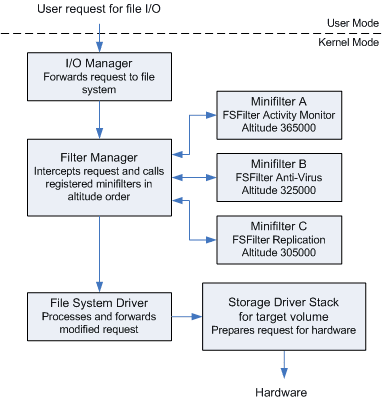
\includegraphics[scale=0.6]{figures/filterDriver.png}}  
	\caption{Simplified I/O stack from Windows \cite{msdn}}
	\label{filterDriver}
\end{figure}

Compared to the previous described technology, which is complex for development and mantaining, \textbf{FileSystemWatcher} is a class from .NET that makes file system monitoring straightforward to implement. According to \cite{dotNetFramework}, this class represents a wrapper over Win32 SDK \textit{ReadDirectoryChangesW} function, which is also used by Windows Explorer to monitor folder changes. By being provided by .NET, it is clear, that FileSystemWatcher can be used in User-Mode for development (see Figure \ref{netFramework}). 

\begin{figure}[H]
	\centerline{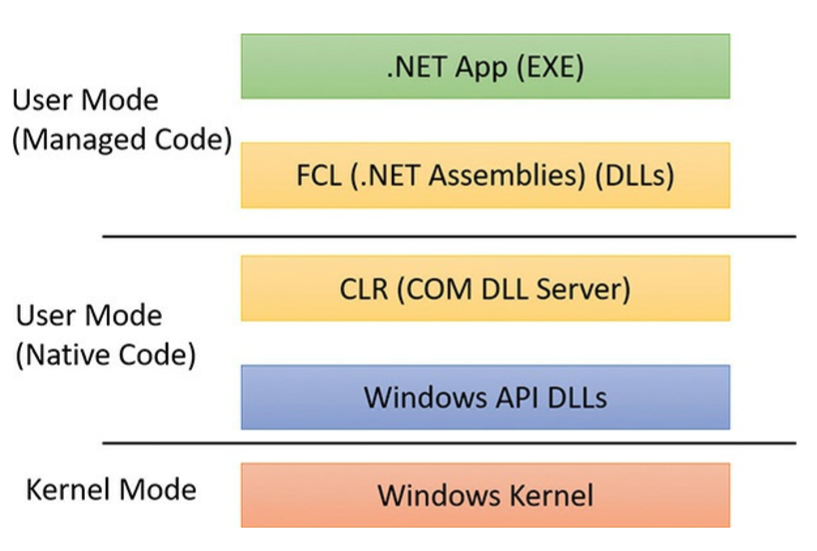
\includegraphics[scale=0.5]{figures/NetFramework.png}}  
	\caption{Relationship between .NET and Windows OS \cite{winInternals}}
	\label{netFramework}
\end{figure}

To configure a working instance of this class, we need to specify a couple of properties, such as \textit{Path} (for indicating the folder to monitor), \textit{NotifyFilters} (for specifieng what kind of file changes to monitor) and \textit{EnableRaisingEvents} (to start/stop monitoring process). Also we need to attach the corresponding events that we want to receive (see Table \ref{table:supportedEvents}).

\begin{table}[H]
	\caption{Events supported by FileSystemWatcher}
	\label{table:supportedEvents}
		\centering
            \begin{tabular}{l | l}
                
				\textbf{Event} & \textbf{Occuring time} \\
				\hline 
 				Created & When a new file is created or is moved into monitored folder \\
 				Changed & When a file has its content or file attributes modified \\
 				Deleted & When a file is removed or is moved out of monitored folder \\
                Renamed & When the name of the file get changed\\
                 
			\end{tabular}
\end{table}

Earlier we mentioned that minifilter drivers live in Kernel-Mode, while FileSystemWatcher provided by .NET lives in User-Mode. One more argument in favor of FileSystemWatcher, besides the high level object-oriented programming language \CSharp that we have at our disposal over unmanaged\footnote{code executed directly by OS; does not provide any security to the application} C language, is that it's safer to run applications in User-Mode. Each application runs in isolation in User-Mode and in case of a crash, it won't affect other applications or even worse the OS itself, what can happen with a Kernel-Mode driver. Even the smallest error that occurs in a driver can cause BSOD\footnote{"Blue Screen of Death", error screen displayed by Windows in case of fatal system crash}. 

\newpage
\section{Analyzing PDF File Structure}
\label{section:pdfStructure}
In this section we are going to understand PDF structure which is a foundation stone of identifieng backdoors\footnote{a malicious method by which a system bypass is hidden} in this file format. \par
PDF was first developed by Adobe in the 1990's with many version been released afterwards. Its initial purpose was to allow to present various types of data, including: text, images, webpage links etc. regardless of the environments it was opened in. As explained in \cite{pdfReference}, PDF files consist of objects, which are of eight types: Boolean values, Numbers (integer and real), Strings, Names, Arrays, Dictionaries, Streams and the Null object. Each PDF document should begin with a header that identifies it as a \textit{PDF} and includes the version number \code{\%PDF-1.7}. The document should also end in a certain way - with the signature \code{\%\%EOF}. After the header the objects are declared.



\begin{figure}[H]
	\centerline{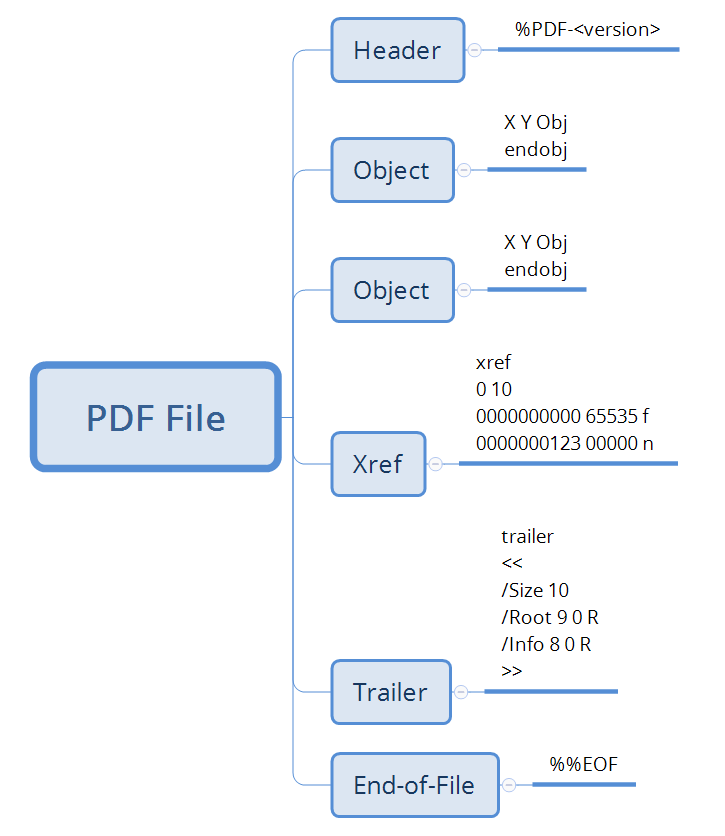
\includegraphics[scale=0.4]{figures/PDFSkeleton.png}}  
	\caption{Structure of PDF Format \cite{winInternals}}
	\label{pdfSkeleton}
\end{figure}


\section{Malware in PDF}
\label{section:malwareInPDF}
% Since PDF documents became a well known solution for information sharing, they also became a good target for cybercriminals.

\section{Machine Learning for Malware Detection}
\label{section:mlForMalware}

\section{Benefits of Cloud Computing}
\label{section:cloudComputing}
% Using a cloud-based anti-virus makes it much easier to manage, especially as there's no need to constantly update software on multiple devices. However, it is worth bearing in mind that installing anti-virus to combat malware can only be one part of an overall IT security policy.
% https://www.redhat.com/en/topics/cloud-native-apps/what-are-cloud-applications
% Simply put, a cloud application is software that users access primarily through the internet, meaning at least some of it is managed by a server, not the user’s local machine. This basic definition doesn’t fully describe how cloud applications have reshaped markets and business models, though. If designed well, cloud applications can offer a user experience like a program installed entirely on a local machine, but with reduced resource needs, more convenient updating, and the ability to access functionality across different devices.
% Nowadays with cloud use being common, it's more efficient to install anti-virus software on your network.
% benfetis - low performant devices + mobile
% http://lxiao.xmu.edu.cn/Papers/Mobile%20Offloading%20for%20Cloud-based%20Malware%20Detections%20with%20Learning.pdf
%Advantages:
% Fast computation to run more advanced and complex detection algorithms
% More accurate detection with a large-size signature database
% Address zero-day vulnerabilitie
% Cloud-based malware detection vs. local detection
%  Transmission delay, computation speed, detection accuracy, storage cost
%  User competition vs. cooperation in the malware detection
%  Compete for the limited network bandwidth
%  Contribute the malware signature database to improve the malware
%  detection accuracy at the cloud
%Cloud computation resource=1Gbps
% Trace generation speed=1Mbps
% Transmission cost factor=0.2
% Accuracy coefficient=0.5 